\lecture{7}{18 Apr 2023 (Zoom)}{Linear Transformation and Matrices}

\begin{recall}
    \begin{enumerate}
        \item[]
        \item \(\psi \in \Hom_\bbk(\bbk^r, V)\) corresponds to \(r\) vectors: \(v_1, v_2, \dots, v_r\):
              \begin{align*}
                  (\psi: \bbk^r \to V)                                      & \rightarrow \{v_i\} = \{\psi(0, \dots, 1, \dots, 0)\} \:\text{(1 in \(i-\)th position)}\: \\
                  \left(\psi: (a_1, a_2, \dots, a_r\right) \to \sum a_iv_i) & \leftarrow \{v_i\}
              \end{align*}
        \item \(V\) has dimension \(d \Leftrightarrow V\) has basis \(\{v_1, v_2, \dots, v_d\}\)
        \item \(\psi: V \xrightarrow{\sim} W\) then \(\psi\) sends a set of basis \(\{v_i\}_{1\leq i \leq d}\) to a set of basis \(\psi(v_i)\) of \(W\)
    \end{enumerate}
\end{recall}

\begin{proof} {Recall 3}
    \textbf{Approach 1}

    One might first prove this statement from first principles, that is to show that:
    \begin{enumerate}
        \item \(\{w_i = \psi(v_i)\}\) span \(W\)
        \item \(\{w_i = \psi(v_i)\}\) are linearly independent
    \end{enumerate}
    This approach is doable, though a little bit tedious.

    \textbf{Approach 2}

    Observe that \(\{v_i\}\) corresponds to a map:

    \[
        \bbk^d \xrightarrow{\sim} V
    \]

    while \[
        V \xrightarrow[\psi]{\sim} W
    \]
    by assumption.

    It then follows that \(\bbk^d \xrightarrow{\sim} W\), following the function composition, it would yield that this mapping corresponds to \(\{w_i = \psi(v_i)\}\). Therefore \(\{w_i\}\) forms a basis of \(W\).
\end{proof}

\subsection{Linear Transformation as Matrix Multiplication}
\begin{claim}
    Let \(V, W\) be vector spaces over \(\bbk\) of dimensions \(n, m\) respectively. Let \(\psi: V \to W\) be a linear transformation. Then once we've fixed bases \(\{v_i\}_{1\leq i \leq n}\) of \(V\) and \(\{w_j\}_{1 \leq j \leq m}\) of \(W\), \(\psi\) corresponds to \(T_\psi \in \bbm_{m\times n}(\bbk)\)

    In other words, \[
        \psi \in \Hom_\bbk(V, W) \leftrightarrow T_\psi \in \bbm_{m\times n}(\bbk)
    \]
\end{claim}
Specifically,
\[
    T_\psi = (\alpha_{ji}) = \begin{pmatrix}
            \alpha_{11} & \alpha_{12} & \cdots & \alpha_{1n} \\
            \vdots      & \vdots      & \ddots & \vdots      \\
            \alpha_{m1} & \alpha_{m2} & \cdots & \alpha_{mn}
        \end{pmatrix}
\]
corresponds to \[
    \psi: v_i \mapsto \alpha_{1i}w_1 + \alpha_{2i}w_2 + \cdots + \alpha_{mi}w_m = \sum_{j=1}^{m}\alpha_{ji} w_j \:\text{for \(1 \leq i \leq n\)}\:
\]

For any \(v = \sum_{i = 1}^{n}\beta_i v_i \in V\) then \begin{align*}
    w = \psi(v) & = \sum_{i=1}^{n} \beta_i \psi(v_i)                                 \\
                & = \sum_{i=1}^{n} \beta_i \left(\sum_{j=1}^{m}\alpha_{ji}w_j\right) \\
                & = \sum_{i=1}^{n}\sum_{j=1}^{m}\alpha_{ji} \beta_i w_j
\end{align*}

An alternative perspective is that \(
v = \sum_{i=1}^{n} \beta_i v_i
\) can be thought of as a ``matrix'' multiplication: \[\begin{pmatrix}
            \beta_1 \\ \vdots \\ \beta_n
        \end{pmatrix} (v_1 \ldots v_n)\]

where \(\begin{pmatrix}
        \beta_1 \\ \vdots \\ \beta_n
    \end{pmatrix} \in \bbm_{n \times 1}(\bbk)\) and \((v_1 \ldots v_n)\) is just the basis in the row vector form.

(Warning: It is not a matrix, since \(v_i \not \in \bbk\))

\textbf{Upshot:} If we fix basis \(v_1, v_2, \dots, v_n\) then any \(v \in V\) would be uniquely expressed as \(v = \beta_i v_i\). The fixed basis would then correspond to unique matrices \(\begin{pmatrix}
        \beta_1 \\ \vdots \\ \beta_n
    \end{pmatrix} \in \bbm_{n \times 1}(\bbk)\)

Note that if we change the basis to another \(\{v'_i\}\) then \[
    v = \sum \beta_i v_i = \sum \beta'_i v'_i \:\text{where}\:  \begin{pmatrix}
            \beta'_1 \\ \vdots \\ \beta'_n
        \end{pmatrix} \in \bbm_{n \times 1}(\bbk)
\]

Now, if \(T_\psi = (a_{ji})_{1 \leq j \leq m, 1 \leq i \leq n}\) then the map \(\psi\) sends \(v \leftrightarrow \begin{pmatrix}
        \beta_1 \\ \vdots \\ \beta_n
    \end{pmatrix}\) to
\[
    \begin{pmatrix}
            \alpha_{11} & \alpha_{12} & \cdots & \alpha_{1n} \\
            \vdots      & \vdots      & \ddots & \vdots      \\
            \alpha_{m1} & \alpha_{m2} & \cdots & \alpha_{mn}
        \end{pmatrix}
    \begin{pmatrix}
            \beta_1 \\ \vdots \\ \beta_n
        \end{pmatrix} = \begin{pmatrix}
            \sum_{i=1}^{n}\alpha_{1i}\beta_i = \gamma_1 \\
            \sum_{i=1}^{n}\alpha_{2i}\beta_i = \gamma_2 \\
            \vdots                                      \\
            \sum_{i=1}^{n}\alpha_{mi}\beta_i = \gamma_m \\
        \end{pmatrix} \in \bbm_{m \times 1}(\bbk)
\]
which corresponds to writing \(w \in W\) under \(\{w_j\}\) as \begin{align*}
    w & = \gamma_1 w_1 + \cdots + \gamma_m w_m                                              \\
      & = \sum_{j=1}^{m}\gamma_j w_j = \sum_{j=1}^{m} \sum_{i=1}^{n} \alpha_{ji}\beta_i w_j
\end{align*}
which is similar to the expression above.

Therefore, once we choose basis \(\{v_i\}, \{w_j\}\) of \(V, W\) respectively then \(\psi \leftrightarrow T_\psi \in \bbm_{m \times n}(\bbk)\):
\begin{align*}
    v = \sum_{i=1}^{n} \beta_i v_i       & \rightarrow \psi(v) = \sum_{i=1}^{n} \sum_{j=1}^{m} \alpha_{ji} \beta_i v_i \\
    (\alpha_{ji}) \begin{pmatrix}
                                \beta_1 \\ \vdots \\ \beta_n
                            \end{pmatrix} & \leftrightarrow \begin{pmatrix}
                                                                           \gamma_1 \\ \vdots \\ \gamma_m
                                                                       \end{pmatrix}
\end{align*}

\subsection{Going from Linear Transformation to Matrix}
We've successfully represented linear transformation \(\psi \in \Hom_\bbk(V, W)\) from \(T_\psi\). How about the other way around, i.e. we know \(\psi\) and want to find its corresponding matrix \(T_\psi\)?

Consider \(\psi: v_i \to \psi(v_i) \in W = c_1 w_1 + \cdots + c_m w_m\) then we can define \(a_{ji} = c_j\) in this expression. Iterating over \(1 \leq i \leq n\) would yield us \(T_\psi = (a_{ji})\).

\subsubsection{Standard \(\bbk^n \to \bbk^m\)}
We have \(\bbk^n, \bbk^m (\bbk^n = \bbk^{\oplus n} = \{x_1, x_2, \ldots, x_n \mid x_i \in \bbk\})\) then there's a preferred basis \(\{e_i\}_{1 \leq i \leq n}\):
\begin{align*}
    e_1 & = (1, 0, \ldots, 0) \in \bbk^n                                            \\
    e_i & = (0, 0, \ldots, 1, \ldots, 0) \in \bbk^n  \:\text{(\(i-\)th position)}\: \\
        & \vdots                                                                    \\
    e_n & = (0, 0, \ldots, 1) \in \bbk^n
\end{align*}
and similarly for \(e'_j \in \bbk^m\).

Under this basis, \((x_1, x_2, \ldots, x_n)\) corresponds to \(\begin{pmatrix}
        \beta_1 \\ \vdots \\ \beta_n
    \end{pmatrix} = \begin{pmatrix}
        x_1 \\ \vdots \\ x_n
    \end{pmatrix} \in \bbm_{n \times 1}(\bbk)\)

It follows that any linear transformation \(\psi \in \Hom_\bbk(\bbk^n, \bbk^m)\) corresponds to \[T_\psi = (\alpha_{ji}) = \begin{pmatrix}
            \alpha_{11} & \cdots & \alpha_{1n} \\
            \vdots      & \ddots & \vdots      \\
            \alpha_{m1} & \cdots & \alpha_{mn}
        \end{pmatrix}\]
with \(\psi\) sending: \[
    \begin{pmatrix}
            \alpha_{11} & \cdots & \alpha_{1n} \\
            \vdots      & \ddots & \vdots      \\
            \alpha_{m1} & \cdots & \alpha_{mn}
        \end{pmatrix}\begin{pmatrix}
            x_1 \\ \vdots \\ x_n
        \end{pmatrix} = \begin{pmatrix}
            y_1    \\
            \vdots \\
            y_m
        \end{pmatrix}
\]

\subsubsection{General Case \(V \to W\)}
With \(\psi \in \Hom_\bbk(V, W)\), and isomorphisms \(\psi_1: \bbk^n \xrightarrow{\sim} V, \psi_2: \bbk^m \xrightarrow{\sim} W\) with corresopnding bases \(\{v_i\}, \{w_j\}\):
\begin{figure} [H]
    \begin{center}
        \tikzset{every picture/.style={line width=0.75pt}} %set default line width to 0.75pt        
        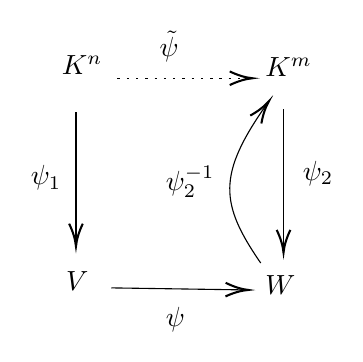
\begin{tikzpicture}[x=0.75pt,y=0.75pt,yscale=-1,xscale=1]
            %uncomment if require: \path (0,300); %set diagram left start at 0, and has height of 300

            %Straight Lines [id:da695871819745131] 
            \draw    (128,101) -- (128,163.5) ;
            \draw [shift={(128,165.5)}, rotate = 270] [color={rgb, 255:red, 0; green, 0; blue, 0 }  ][line width=0.75]    (10.93,-3.29) .. controls (6.95,-1.4) and (3.31,-0.3) .. (0,0) .. controls (3.31,0.3) and (6.95,1.4) .. (10.93,3.29)   ;
            %Straight Lines [id:da656763463540512] 
            \draw    (145,185.5) -- (209,186.47) ;
            \draw [shift={(211,186.5)}, rotate = 180.87] [color={rgb, 255:red, 0; green, 0; blue, 0 }  ][line width=0.75]    (10.93,-3.29) .. controls (6.95,-1.4) and (3.31,-0.3) .. (0,0) .. controls (3.31,0.3) and (6.95,1.4) .. (10.93,3.29)   ;
            %Straight Lines [id:da46225545196828643] 
            \draw    (228,99.5) -- (228,166.5) ;
            \draw [shift={(228,168.5)}, rotate = 270] [color={rgb, 255:red, 0; green, 0; blue, 0 }  ][line width=0.75]    (10.93,-3.29) .. controls (6.95,-1.4) and (3.31,-0.3) .. (0,0) .. controls (3.31,0.3) and (6.95,1.4) .. (10.93,3.29)   ;
            %Straight Lines [id:da17654653607895265] 
            \draw  [dash pattern={on 0.84pt off 2.51pt}]  (148,84.5) -- (211,84.5) ;
            \draw [shift={(213,84.5)}, rotate = 180] [color={rgb, 255:red, 0; green, 0; blue, 0 }  ][line width=0.75]    (10.93,-3.29) .. controls (6.95,-1.4) and (3.31,-0.3) .. (0,0) .. controls (3.31,0.3) and (6.95,1.4) .. (10.93,3.29)   ;
            %Curve Lines [id:da8908595252766036] 
            \draw    (217,173.5) .. controls (197.3,144.93) and (196.03,130.92) .. (219.89,97.06) ;
            \draw [shift={(221,95.5)}, rotate = 125.54] [color={rgb, 255:red, 0; green, 0; blue, 0 }  ][line width=0.75]    (10.93,-3.29) .. controls (6.95,-1.4) and (3.31,-0.3) .. (0,0) .. controls (3.31,0.3) and (6.95,1.4) .. (10.93,3.29)   ;

            % Text Node
            \draw (120,72.4) node [anchor=north west][inner sep=0.75pt]    {$\mathbb{K}^{n}$};
            % Text Node
            \draw (122,176.4) node [anchor=north west][inner sep=0.75pt]    {$V$};
            % Text Node
            \draw (218,178.4) node [anchor=north west][inner sep=0.75pt]    {$W$};
            % Text Node
            \draw (218,73.4) node [anchor=north west][inner sep=0.75pt]    {$\mathbb{K}^{m}$};
            % Text Node
            \draw (105,125.4) node [anchor=north west][inner sep=0.75pt]    {$\psi_1 $};
            % Text Node
            \draw (236,123.4) node [anchor=north west][inner sep=0.75pt]    {$\psi_2 $};
            % Text Node
            \draw (170,193.4) node [anchor=north west][inner sep=0.75pt]    {$\psi $};
            % Text Node
            \draw (167,60.4) node [anchor=north west][inner sep=0.75pt]    {$\tilde{\psi} $};
            % Text Node
            \draw (170,125.4) node [anchor=north west][inner sep=0.75pt]    {$\psi^{-1}_2 $};
        \end{tikzpicture}
    \end{center}
\end{figure}





then \(\psi \in \Hom_\bbk(V, W)\) corresponds to \(\tilde{\psi} \in \Hom_\bbk(\bbk^n, \bbk^m)\)  (through \(\psi_1, \psi_2\)), and this \(\tilde{\psi}\) corresponds to \(T_{\tilde{\psi}}\)!

\begin{exercise}
    Given linear transformation \(\psi: \bbk^n \to \bbk^n\) that corresponds to \(T_\psi \in \bbm_{n \times n}(\bbk)\).

    Show that \(\psi\) is isomorphism \(\Leftrightarrow T_\psi\) is invertible.
\end{exercise}

\begin{remark}
    Consider \(\psi: \bbk^n \to \bbk^m\) that corresponds to matrix \(T_\psi = A = (\alpha_{ji})\). Then,

    \begin{multline*}
        \ker(\psi) = \{v \in \bbk^n \mid \psi(v) = 0\} = \left\{\begin{pmatrix}
                x_1 \\ \vdots \\ x_n
            \end{pmatrix} \in \bbk^n \;\middle|\; A \cdot \begin{pmatrix}
                x_1 \\ \vdots \\ x_n
            \end{pmatrix} = 0 \right\} \\
        = \:\text{null space of}\:A
    \end{multline*}
    \begin{multline*}
        \im(\psi) = \{w \in \bbk^m \mid w = \psi(v) \:\text{ for some }\: v\} = \left\{\begin{pmatrix}
                y_1 \\ \vdots \\y_n
            \end{pmatrix} = A \cdot \begin{pmatrix}
                x_1 \\ \vdots \\ x_n
            \end{pmatrix} \:\text{for some}\: \{x_1, \dots, x_n\}\right\} \\
            = \:\text{range of}\: A
    \end{multline*}
\end{remark}

\begin{recall}
    Relating the this with a previous dimensional equality:
    \begin{align*}
        \dim_\bbk \bbk^n &= n \\
        &= \dim_\bbk (\im(\psi)) + \dim_\bbk (\ker(\psi))\\
        &= \:\text{rank of}\: A + \:\text{nullity of}\: A
    \end{align*}
\end{recall}

\subsection{Determinant}

Determinant is simply a function \(D: \bbm_{n \times n}(\bbk) \to \bbk\)

\begin{definition} {Multilinearity and Alternating}
    A function \(f: \bbm_{n \times n}(\bbk) \to \bbk\) is called \textbf{multilinear} if the following holds:

    Given \(A = \begin{pmatrix}
    r_1 \\ \vdots \\ r_n
    \end{pmatrix}\) where row \(r_i = (a_{i1} \: a_{i2} \: \ldots \: a_{in})\), \[
    f \begin{pmatrix}
    r_1 \\ \vdots \\ \alpha r_i + \beta r'_i \\ \vdots \\ r_n
    \end{pmatrix} = \alpha f \begin{pmatrix}
    r_1 \\ \vdots \\ r_i \\ \vdots \\ r_n 
    \end{pmatrix} + \beta f \begin{pmatrix}
    r_1 \\ \vdots \\ r'_i \\ \vdots \\ r_n
    \end{pmatrix} \:\text{where}\: \alpha, \beta \in \bbk
    \]

    \(f\) is \textbf{alternating} if the following holds:
    \begin{enumerate}
        \item \(f \begin{pmatrix}
            r_1 \\ \vdots \\ r_n
            \end{pmatrix} = 0\) whenever \(\exists r_i = r_j, i \neq j\)
            \item \(f \begin{pmatrix}
            r_1 \\ \vdots \\ r_i \\ r_{i+1}\\ \vdots \\ r_n
            \end{pmatrix} = -f \begin{pmatrix}
                r_1 \\ \vdots \\ r_{i+1}\\ r_i \\ \vdots \\ r_n
                \end{pmatrix} \) 
    \end{enumerate}
\end{definition}

\begin{remark}
    If \(2 \neq 0\) in \(\bbk\) then the second condition for alternating implies the first one.
\end{remark}

\begin{definition} {Determinant}
    A \textbf{determinant} function \(\bbm_{n \times n}(\bbk)\) is a multilinear and alternating function \(D: \bbm_{n \times n}(\bbk) \to \bbk\) \st \(D(I_n) = 1\)
\end{definition}

\begin{remark}
    For each \(n\) there is a unique determinant function \(\bbm_{n\times n}(\bbk)\), usually written as \(\det\). To be discussed further next lecture.
\end{remark}